\documentclass[submit]{harvardml}

% Put in your full name and email address.
\name{Matthew Leifer}
\email{matthewleifer@college.harvard.edu}

% List any people you worked with.
\collaborators{%
	John Doe,
	Fred Doe
}

% You don't need to change these.
\course{CS181-S17}
\assignment{Assignment \#4}
\duedate{5:00pm March 31, 2017}

\usepackage[OT1]{fontenc}
\usepackage[colorlinks,citecolor=blue,urlcolor=blue]{hyperref}
\usepackage[pdftex]{graphicx}
\usepackage{subfig}
\usepackage{fullpage}
\usepackage{amsmath}
\usepackage{amssymb}
\usepackage{tikz}
\usetikzlibrary{fit,positioning}
\usetikzlibrary{bayesnet}
\usepackage{color}
\usepackage{todonotes}
\usepackage{listings}
\usepackage{common}
\usepackage{bm}


\usepackage[mmddyyyy,hhmmss]{datetime}

\definecolor{verbgray}{gray}{0.9}

\lstnewenvironment{csv}{%
	\lstset{backgroundcolor=\color{verbgray},
		frame=single,
		framerule=0pt,
		basicstyle=\ttfamily,
		columns=fullflexible}}{}

\begin{document}
	\begin{center}
		{\Large Homework 4: Clustering and EM}\\
	\end{center}
	
	
	This homework assignment focuses on different unsupervised learning
	methods from a theoretical and practical standpoint.  In Problem 1, you
	will explore Hierarchical Clustering and experiment with how the
	choice of distance metrics can alter the behavior of the algorithm. In
	Problem 2, you will derive from scratch the full
	expectation-maximization algorithm for fitting a simple topic
	model. In Problem 3, you will implement K-Means clustering on a
	dataset of handwritten images and analyze the latent structure learned by 
	this algorithm.
	
	
	
	There is a mathematical component and a programming component to this homework.
	Please submit your PDF and Python files to Canvas, and push all of your work to your GitHub
	repository. If a question requires you to make any plots, please
	include those in the writeup.
	
	
	
	\newpage
	\section*{Hierarchical Clustering [7 pts]}
	
	At each step of hierarchical clustering, the two most similar clusters
	are merged together. This step is repeated until there is one single
	group. We saw in class that hierarchical clustering will return a
	different result based on the pointwise-distance and cluster-distance
	that is is used. In this problem you will examine different choices of
	pointwise distance (specified through choice of norm) and cluster
	distance, and explore how these choices change how the HAC algorithm
	runs on a toy data set.
	
	
	\vspace{0.25cm}
	
	\begin{problem}
		~
		
		Consider the following four data points in $\reals^2$, belonging to three clusters: the
		black cluster consisting of $\boldx_1 = (0.1, 0.5) $ and $\boldx_2 = (0.35, 0.75))$,
		the red cluster consisting of $\boldx_3 = (0.28, 1.35)$, and the blue cluster
		consisting of $\boldx_4 = (0, 1.01)$.
		
		\begin{center} 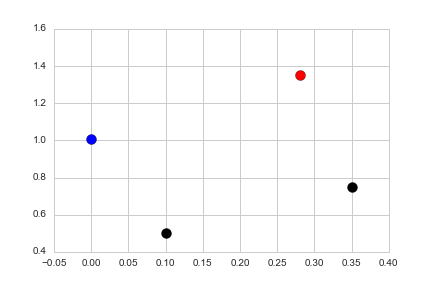
\includegraphics[scale=.3]{scatterplot.png} \end{center}
		
		
		Different pointwise distances $d(\boldx, \boldx') = \|\boldx - \boldx'\|_p$
		can be used.  Recall the definition of the
		$\ell_1$, $\ell_2$, and $\ell_{\infty}$ norm:
		\begin{eqnarray*}
			\| \mathbf{x} \|_1 = \sum_{j = 1}^m |x_i| \quad \quad\quad \| \mathbf{x} \|_2 = \sqrt{\sum_{j = 1}^m x_i^2 } \quad\quad\quad
			\| \mathbf{x} \|_{\infty} = \max_{j \in \{1, \ldots, m\}} |x_j|\\
		\end{eqnarray*}
		
		
		Also recall the definition of min-distance, max-distance,
		centroid-distance, and average-distance between two clusters (where $\bmu_{G}$
		is the center of a cluster $G$):
		%
		\begin{eqnarray*}
			d_{\text{min}}(G, G') &=& \min_{\boldx  \in G, \boldx' \in G'} d(\boldx, \boldx')\\
			d_{\text{max}}(G, G') &=& \max_{\boldx  \in G, \boldx' \in G'} d(\boldx, \boldx')\\
			d_{\text{centroid}}(G, G') &=&  d(\bmu_{G}, \bmu_{G'})\\
			d_{\text{avg}}(G, G') &=&\frac{1}{|G| |G'|} \sum_{\boldx \in G}\sum_{\boldx'  \in G'} d(\boldx, \boldx')\\
		\end{eqnarray*}
		
		\begin{enumerate}
			\item Draw the 2D unit sphere for each norm,
			defined as $\mathcal{S} = \{\boldx \in \mathbb{R}^2: \|\boldx\| = 1 \}$. Feel free to do
			it by hand, take a picture and include it in your pdf.
			\item  For each norm ($\ell_1, \ell_2, \ell_\infty$) and each clustering distance, specify which two clusters would
			be the first to merge.
			\item Draw the complete dendrograms showing the order of agglomerations for the $\ell_2$ norm and each of the clustering distances.
		\end{enumerate}
		
		
	\end{problem}
	
	\subsection*{Solution}
	
	\begin{enumerate}
		
		\item The top left is the $\ell_1$ norm unit circle, the right most graph is the $\ell_2$ unit circle and the bottom most graph is the $\ell_\infty$ unit circle.  \\ 
		
		\includegraphics[width=0.5\textwidth]{IMG_2122.JPG}
		
		\item Here's a table displaying the first two clusters two merge based on different metrics and norms: \\
		\begin{tabular}{l | c | r}
			
			Norm & Distance & Clusters Merge \\
			\hline
			$\ell_1$ & $d_{min}$ & Black and blue \\
			$\ell_1$ & $d_{max}$ & Black and blue \\
			$\ell_1$ & $d_{centroid}$ & Black and blue \\
			$\ell_1$ & $d_{avg}$ & Black and blue \\
			
			$\ell_2$ & $d_{min}$ & Black and blue \\
			$\ell_2$ & $d_{max}$ & Red and blue \\
			$\ell_2$ & $d_{centroid}$ & Red and blue \\
			$\ell_2$ & $d_{avg}$ & Red and blue \\
			
			$\ell_\infty$ & $d_{min}$ & Red and blue \\
			$\ell_\infty$ & $d_{max}$ & Red and blue \\
			$\ell_\infty$ & $d_{centroid}$ & Red and blue \\
			$\ell_\infty$ & $d_{avg}$ & Red and blue \\
			
		\end{tabular}
		
		\item Here is an image of the dendrograms: \\
		\includegraphics[width=0.5\textwidth]{IMG_2139.jpg}
	\end{enumerate}
	
	
	
	\newpage 
	\section*{Topic Modeling [15 pts]}
	
	
	In this problem we will explore a simplified version of topic
	modeling in which each document has just a \textit{single} topic.
	For this problem, we will assume there are $c$~topics. Each topic $k \in \{1, \ldots, c\}$ will be
	associated with a vector $\bbeta_k \in [0,1]^{|\mcV|}$ describing a
	distribution over the vocabulary $\mcV$ with
	${\sum_{j=1}^{|\mcV|} \beta_{k,j}=1}$.
	
	Each document $\boldx_i$ will represented as a
	bag-of-words~$\boldx_{i} \in (\mathbb{Z}^{\geq 0})^{|\mcV|}$, where~$x_{i,j}$ is a
	non-negative integer representing the number of times word $j$ appeared in document $i$.  Document~$i$ has~$n_i$
	word tokens in total. Finally let the (unknown) overall mixing
	proportion of topics be~$\btheta \in [0,1]^c$,
	where~${\sum_{k=1}^c \theta_k=1}$.
	
	Our generative model is that each of the~$n$ documents has a single
	topic. We encode this topic as a one-hot
	vector~${\boldz_i \in \{0,1\}^c}$ over topics. This one-hot vector is
	drawn from~$\btheta$; then, each of the words is drawn
	from~$\bbeta_{z_i}$. Formally documents are generated in two steps:
	\begin{eqnarray*}
		\boldz_i &\sim& \text{Categorical}(\btheta) \\
		\boldx_i &\sim& \text{Multinomial}(\bbeta_{\boldz_i})   
	\end{eqnarray*}
	
	
	\begin{problem}
		~
		
		\begin{enumerate}
			\item Draw the graphical model representation of this 
			problem. Be sure to use the plate notation to 
			indicate repeated random variables and gray nodes 
			to indicate observed variables.
			
			\item \textbf{Complete-Data Log Likelihood} Define the complete data for this problem to be $D = \{(\boldx_i, \boldz_i)\}_{i=1}^n$. 
			\begin{itemize}
				\item Write out the complete-data (negative) log likelihood. \[\mcL(\btheta, \{\bbeta_k\}^c_{k=1}) =  -\ln p(D \given\btheta, \{\bbeta_k\}^c_{k=1}).\] 
				\item Explain in one sentence why we cannot directly optimize this loss function.
			\end{itemize}
			
			
			
			\item \textbf{Expectation Step}
			Our next step is to introduce a mathematical expression for $\boldq_i$, the posterior over the hidden topic variables~$\boldz_i$ conditioned on the observed data $\boldx_i$ with fixed parameters, i.e $p(\boldz_i | \boldx_i; \btheta, \{\bbeta_k\}^c_{k=1})$.
			
			\begin{itemize}
				\item  Write down and simplify the expression for $\boldq_i$. 
				\item  Give an algorithm for calculating $\boldq_i$ for all $i$, given the observed data~$\{\boldx_i\}^n_{i=1}$ and settings of the parameters~$\btheta$ and~$\{\bbeta_k\}^c_{k=1}$.
				
			\end{itemize}
			
			\item \textbf{Maximization Step}
			Using the~$\boldq_i$ estimates from the Expectation Step, derive an update for maximizing the expected complete data log likelihood in terms of~$\btheta$ and~$\{\bbeta_k\}^c_{k=1}$.
			
			\begin{itemize}
				\item Derive an expression for the expected complete-data log likelihood in terms of $\boldq_i$.
				\item Find an expression for $\btheta$ that maximizes this expected complete-data log likelihood. You may find it helpful to use Lagrange multipliers in order to force the constraint $\sum \theta_k = 1$. Why does this optimized $\btheta$ make intuitive sense?
				\item Apply a similar argument to find the value of the $\bbeta_{k}$'s that maximizes the expected complete-data log likelihood. 
			\end{itemize}
		\end{enumerate}
		
	\end{problem}
	
	\subsection*{Solution}
	
	\begin{enumerate}
		\item
		\begin{figure}
			\centering
			\tikz{ %
				\node[latent] (theta) {$\btheta$} ; %
				\node[latent, below=of theta] (z) {$\boldz_i$} ; %
				\node[latent, right=of z] (beta) {$\beta_k$} ; %
				\node[obs, below=of z] (x) {$\boldx_i$} ; %
				\plate[inner sep=0.25cm, xshift=-0.12cm, yshift=0.12cm] {plate1} {(z) (x)} {n}; %
				\plate[inner sep=0.25cm, xshift=-0.12cm, yshift=0.12cm] {plate2} {(beta)} {c}; %
				\edge {theta} {z} ; %
				\edge {z,beta} {x} ; %
			}
		\end{figure}
		
		\item \[\mcL(\btheta, \{\bbeta_k\}^c_{k=1}) =  
		-\ln p(D \given\btheta, \{\bbeta_k\}^c_{k=1}) = 
		-\ln \prod_{i = 1}^np(\boldx_i, \boldz_i = C_k | \btheta, \{B_k\}_{k=1}^c) = \]
		\[
		-\ln \displaystyle\prod_{i = 1}^{n}\prod_{j = 1}^{|\mcV|}\beta_{z_{ij}}^{x_{ij}}\theta_k =
		\sum_{i = 1}^{n}\sum_{j = 1}^{|\mcV|}\ln\theta_k+x_{ij}\ln\beta_{z_ij}\]
		
		We can't optimize this loss funciton directly because we don't know what $z_i$ is - it's a latent variable. 
		\item \[ q_{ik} = 
		p(z_i = C_k | x_i; \btheta, \{\beta_k\}_{k = 1}^c) \propto \]
		\[
		p(\boldx | z_i = C_k; \theta, \{\beta_k\}_{k=1}^c)p(z_i = C_k | \btheta, \{\beta_{k = 1}^c\}) = 
		\prod_{j = 1}^{|\mcV|}\beta_{z_ij}^{x_{ij}}\theta_k
		\]
		And then to actually calculate $\boldq_i$ and not just something proportional to it, calculate all of those probabilities and take their sum and divide each term found above by that.  
		
		\[
		q_{ik} = \dfrac{\prod_{j = 1}^{|\mcV|}\beta_{z_ij}^{x_{ij}}\theta_k}{\sum_{m=1}^{c}\prod_{j = 1}^{|\mcV|}\beta_{z_ij}^{x_{ij}}\theta_m}
		\]
		
		In order to actually calculate $\boldq_i$, I'd first initialize $\btheta$ and $\{\beta_k\}_k$ randomly, making sure that they don't start out as uniform distributions, because otherwise it'll just be stuck.  Then with those values, I would be able to calculate the distribution of $\boldq$ over $\boldz$.  Then using these $\boldq_i$'s I would update $\btheta$ and $\{\beta_k\}_k$ such that the expected complete log likelihood of the data is maximized, repeating these steps until the log likelihood converges.  
		
		\item Given all this, the expected complete data log likelihood of the data is $\displaystyle\sum_{i = 1}^{n}\sum_{k = 1}^{c}q_{ik}(\ln\theta_k + \sum_{j = 1}^{|\mcV|}x_{ij}\ln\beta_{kj})$ \\
		
		Since I'm going to optimize with respect to $\theta$, I dropped all the terms that didn't depend on $\theta$ \\
		\[\mcL(\theta,\lambda) = -\displaystyle\sum_{i = 1}^{n}\sum_{k = 1}^{c}q_{ik}\ln\theta_k + \lambda(\sum_{m=1}^{c}\theta_m - 1)\] \\
		\[ \dfrac{\partial\mcL}{\partial\theta_k} = - \sum_{i=1}^{n}q_{ik}\cdot\frac{1}{\theta_k} + \lambda = 0 \] \\
		\[ \lambda = \dfrac{1}{\theta_k}\sum_{i =1}^{n}q_{ik}   \]
		\[ \theta_k = \frac{1}{\lambda}\sum_{i=1}^{n}q_{ik}\] 
		Sum both sides over $k$ \\
		\[ 1 = \frac{1}{\lambda} \sum_{i = 1}^{n}\sum_{k=1}^{c}q_{ik}\]
		\[\lambda = \sum_{i = 1}^{n}\sum_{k=1}^{c}q_{ik} \]
		\[\hat{\theta_k} = \frac{1}{n}\sum_{i = 1}^{n}q_{ik}\]
		
		This optimized $\btheta$ makes sense because each entry which represents the probability that a document is in class $k$ is the average of the posterior probabilities across all the data points that a document is in class $k$ which seems reasonable.  \\
		
		\[\mcL(\beta, \lambda) = -\sum_{i = 1}^n\sum_{k = 1}^{c}q_{ik}\sum_{j = 1}^{|\mcV|}x_{ij}\ln\beta_{kj} + \lambda(\sum_{k = 1}^{c}\sum_{j = 1}^{|\mcV|}\beta_{kj} - 1) \]
		
		\[\dfrac{\partial\mcL(\beta,\lambda)}{\partial\beta_{kj}} = -\sum_{i=1}^{n}\dfrac{q_{ik}x_{ij}}{\beta_{kj}} + \lambda = 0\]
		\[\lambda = \sum_{i = 1}^{n}\dfrac{q_{ik}x_{ij}}{\beta_{kj}}   \] 
		\[\sum_{j = 1}^{|\mcV|}\beta_{kj} = \frac{1}{\lambda} \sum_{i=1}^{n}\sum_{j = 1}^{|\mcV|}q_{ik}x_{ij} \]
		\[\lambda = \sum_{i=1}^{n}\sum_{j = 1}^{|\mcV|} q_{ik}x_{ij}\]
		\[\hat{\beta_{kj}} = \dfrac{\displaystyle\sum_{i = 1}^{n}q_{ik}x_{ij}}{\displaystyle\sum_{i=1}^{n}\sum_{j = 1}^{|\mcV|}q_{ik}x_{ij}}\]
	\end{enumerate}
	
	
	\newpage
	
	\section*{K-Means [15 pts]}
	
	For this problem you will implement  K-Means clustering from scratch. Using \texttt{numpy} is fine, but don't use a
	third-party machine learning implementation like \texttt{scikit-learn}. You will then apply this approach to clustering of image data.  
	
	
	
	We have provided you with the MNIST dataset, a collection of handwritten digits used as a benchmark of image recogntion (you  can
	learn more about the data set at  \url{http://yann.lecun.com/exdb/mnist/}). The MNIST task
	is widely used in supervised learning, and modern algorithms with neural
	networks do very well on this task. 
	
	Here we will use MNIST unsupervised learning. You have been given
	representations of 6000 MNIST images, each of which are $28\times28$
	greyscale handwritten digits. Your job is to implement K-means
	clustering on MNIST, and to test whether this relatively simple algorithm can
	cluster similar-looking images together.
	
	~
	
	\begin{problem}
		The given code loads the images into your environment as a 6000x28x28 array.
		
		\begin{itemize}
			\item Implement K-means clustering
			from different random initializations 
			and for several values of $K$ using the 
			$\ell_2$ norm as your
			distance metric. (You should feel free to explore other metrics 
			than the $\ell_2$ norm, but this is strictly optional.)  Compare the 
			K-means objective for different values of K and across random
			initializations.
			%
			\item For three different values of K,
			and a couple of random restarts for each, 
			show the mean images for each cluster (i.e., for
			the cluster prototypes), as well as the images for a 
			few representative images for each cluster. You should explain how you selected
			these representative images. To render an image, use the pyplot \texttt{imshow} function. 
			
			\item Are the results wildly different for different
			restarts and/or different 
			values of K?
			For one of your runs, plot the K-means objective function as a function of iteration and verify that
			it never increases.
			
			%\item Finally, implement K-means++ and see if gives you more satisfying
			%initializations (and final results) for K-means. Explain your findings.
			
		\end{itemize}
		
		
		As in past problem sets, please include your plots in this
		document. (There may be several plots for this problem, so feel free
		to take up multiple pages.)
		
		
		
		
	\end{problem}
	\subsection*{Solution}
	
	For the values of $k$ that I tested ($k = 10, k = 11, k = 16$) the loss at the beginning of the trials when using K-means++ was approximately 10 million - of course due to the randomization there was some variation in the intial average.  After running K-means to convergence the value of the objective function decreased to around 9 million.  The results aren't too different for different values of $k$ - K means performs pretty well on clustering similar images.  4's, 9's and 7's are often grouped together and so are 3's and 8's.  5's have a decent amount of variability in how they're written and so they might be grouped with 2's or 3's and are harder to classify. For $k=10$, 5's don't seem to belong to a particular cluster instead, my classifier has two classes for the number 1 - the 1's in one cluster are straight up and in the other are slanted significantly. For $k = 11$ this no longer seems to be a problem and the cluster of slanted 1's has disappeared.  \\\\
	I selected the images that are representative of a cluster by finding the images that were closest (in terms of Euclidean distance) to the mean of that cluster.  I calculated the loss at every iteration and it almost always decreases, however on occasion the loss increases by a very small fraction less than $10^{-6}$.  A TF upon reviewing my code told me that this was just due to floating point imprecision because it's such a small value - can't even be noticed in the loss graph.  \\
	
	This first batch of plots is for $k$ = 10. The large image to the right of the groups of 4 represents the mean for that particular cluster and the group of 4 are the 4 images which are closest to the mean witihin that cluster. \\
	\includegraphics[scale=.25]{Trial_1;_K_=_10;_D_=_4/Cluster_0_Images.png}
	\includegraphics[scale=.25]{Trial_1;_K_=_10;_D_=_4/Mean_for_Cluster_0.png}
	\includegraphics[scale=.25]{Trial_1;_K_=_10;_D_=_4/Cluster_1_Images.png}
	\includegraphics[scale=.25]{Trial_1;_K_=_10;_D_=_4/Mean_for_Cluster_1.png}
	\includegraphics[scale=.25]{Trial_1;_K_=_10;_D_=_4/Cluster_2_Images.png}
	\includegraphics[scale=.25]{Trial_1;_K_=_10;_D_=_4/Mean_for_Cluster_2.png}
	\includegraphics[scale=.25]{Trial_1;_K_=_10;_D_=_4/Cluster_3_Images.png}
	\includegraphics[scale=.25]{Trial_1;_K_=_10;_D_=_4/Mean_for_Cluster_3.png}
	\includegraphics[scale=.25]{Trial_1;_K_=_10;_D_=_4/Cluster_4_Images.png}
	\includegraphics[scale=.25]{Trial_1;_K_=_10;_D_=_4/Mean_for_Cluster_4.png}
	\includegraphics[scale=.25]{Trial_1;_K_=_10;_D_=_4/Cluster_5_Images.png}
	\includegraphics[scale=.25]{Trial_1;_K_=_10;_D_=_4/Mean_for_Cluster_5.png}
	\includegraphics[scale=.25]{Trial_1;_K_=_10;_D_=_4/Cluster_6_Images.png}
	\includegraphics[scale=.25]{Trial_1;_K_=_10;_D_=_4/Mean_for_Cluster_6.png}
	\includegraphics[scale=.25]{Trial_1;_K_=_10;_D_=_4/Cluster_7_Images.png}
	\includegraphics[scale=.25]{Trial_1;_K_=_10;_D_=_4/Mean_for_Cluster_7.png}
	\includegraphics[scale=.25]{Trial_1;_K_=_10;_D_=_4/Cluster_8_Images.png}
	\includegraphics[scale=.25]{Trial_1;_K_=_10;_D_=_4/Mean_for_Cluster_8.png}
	\includegraphics[scale=.25]{Trial_1;_K_=_10;_D_=_4/Cluster_9_Images.png}
	\includegraphics[scale=.25]{Trial_1;_K_=_10;_D_=_4/Mean_for_Cluster_9.png}
	\includegraphics[scale = 0.4]{Trial_1;_K_=_10;_D_=_4/Loss_for_K_=_10.png} 
	\\\\

	Here are the images and clusters for $k$ = 11. \\
	\includegraphics[scale=.25]{Trial_2;_K_=_11;_D_=_4/Cluster_0_Images.png}
	\includegraphics[scale=.25]{Trial_2;_K_=_11;_D_=_4/Mean_for_Cluster_0.png}
	\includegraphics[scale=.25]{Trial_2;_K_=_11;_D_=_4/Cluster_1_Images.png}
	\includegraphics[scale=.25]{Trial_2;_K_=_11;_D_=_4/Mean_for_Cluster_1.png}
	\includegraphics[scale=.25]{Trial_2;_K_=_11;_D_=_4/Cluster_2_Images.png}
	\includegraphics[scale=.25]{Trial_2;_K_=_11;_D_=_4/Mean_for_Cluster_2.png}
	\includegraphics[scale=.25]{Trial_2;_K_=_11;_D_=_4/Cluster_3_Images.png}
	\includegraphics[scale=.25]{Trial_2;_K_=_11;_D_=_4/Mean_for_Cluster_3.png}
	\includegraphics[scale=.25]{Trial_2;_K_=_11;_D_=_4/Cluster_4_Images.png}
	\includegraphics[scale=.25]{Trial_2;_K_=_11;_D_=_4/Mean_for_Cluster_4.png}
	\includegraphics[scale=.25]{Trial_2;_K_=_11;_D_=_4/Cluster_5_Images.png}
	\includegraphics[scale=.25]{Trial_2;_K_=_11;_D_=_4/Mean_for_Cluster_5.png}
	\includegraphics[scale=.25]{Trial_2;_K_=_11;_D_=_4/Cluster_6_Images.png}
	\includegraphics[scale=.25]{Trial_2;_K_=_11;_D_=_4/Mean_for_Cluster_6.png}
	\includegraphics[scale=.25]{Trial_2;_K_=_11;_D_=_4/Cluster_7_Images.png}
	\includegraphics[scale=.25]{Trial_2;_K_=_11;_D_=_4/Mean_for_Cluster_7.png}
	\includegraphics[scale=.25]{Trial_2;_K_=_11;_D_=_4/Cluster_8_Images.png}
	\includegraphics[scale=.25]{Trial_2;_K_=_11;_D_=_4/Mean_for_Cluster_8.png}
	\includegraphics[scale=.25]{Trial_2;_K_=_11;_D_=_4/Cluster_9_Images.png}
	\includegraphics[scale=.25]{Trial_2;_K_=_11;_D_=_4/Mean_for_Cluster_9.png}
	\includegraphics[scale=.25]{Trial_2;_K_=_11;_D_=_4/Cluster_10_Images.png}
	\includegraphics[scale=.25]{Trial_2;_K_=_11;_D_=_4/Mean_for_Cluster_10.png} \\
	\includegraphics[scale = 0.4]{Trial_2;_K_=_11;_D_=_4/Loss_for_K_=_11.png} 
	\\\\
	
	Lastly, $k = 16$. \\
	\includegraphics[scale=.25]{Trial_3;_K_=_16;_D_=_4/Cluster_0_Images.png}
	\includegraphics[scale=.25]{Trial_3;_K_=_16;_D_=_4/Mean_for_Cluster_0.png}
	\includegraphics[scale=.25]{Trial_3;_K_=_16;_D_=_4/Cluster_1_Images.png}
	\includegraphics[scale=.25]{Trial_3;_K_=_16;_D_=_4/Mean_for_Cluster_1.png}
	\includegraphics[scale=.25]{Trial_3;_K_=_16;_D_=_4/Cluster_2_Images.png}
	\includegraphics[scale=.25]{Trial_3;_K_=_16;_D_=_4/Mean_for_Cluster_2.png}
	\includegraphics[scale=.25]{Trial_3;_K_=_16;_D_=_4/Cluster_3_Images.png}
	\includegraphics[scale=.25]{Trial_3;_K_=_16;_D_=_4/Mean_for_Cluster_3.png}
	\includegraphics[scale=.25]{Trial_3;_K_=_16;_D_=_4/Cluster_4_Images.png}
	\includegraphics[scale=.25]{Trial_3;_K_=_16;_D_=_4/Mean_for_Cluster_4.png}
	\includegraphics[scale=.25]{Trial_3;_K_=_16;_D_=_4/Cluster_5_Images.png}
	\includegraphics[scale=.25]{Trial_3;_K_=_16;_D_=_4/Mean_for_Cluster_5.png}
	\includegraphics[scale=.25]{Trial_3;_K_=_16;_D_=_4/Cluster_6_Images.png}
	\includegraphics[scale=.25]{Trial_3;_K_=_16;_D_=_4/Mean_for_Cluster_6.png}
	\includegraphics[scale=.25]{Trial_3;_K_=_16;_D_=_4/Cluster_7_Images.png}
	\includegraphics[scale=.25]{Trial_3;_K_=_16;_D_=_4/Mean_for_Cluster_7.png}
	\includegraphics[scale=.25]{Trial_3;_K_=_16;_D_=_4/Cluster_8_Images.png}
	\includegraphics[scale=.25]{Trial_3;_K_=_16;_D_=_4/Mean_for_Cluster_8.png}
	\includegraphics[scale=.25]{Trial_3;_K_=_16;_D_=_4/Cluster_9_Images.png}
	\includegraphics[scale=.25]{Trial_3;_K_=_16;_D_=_4/Mean_for_Cluster_9.png}
	\includegraphics[scale=.25]{Trial_3;_K_=_16;_D_=_4/Cluster_10_Images.png}
	\includegraphics[scale=.25]{Trial_3;_K_=_16;_D_=_4/Mean_for_Cluster_10.png}
	\includegraphics[scale=.25]{Trial_3;_K_=_16;_D_=_4/Cluster_11_Images.png}
	\includegraphics[scale=.25]{Trial_3;_K_=_16;_D_=_4/Mean_for_Cluster_11.png}
	\includegraphics[scale=.25]{Trial_3;_K_=_16;_D_=_4/Cluster_12_Images.png}
	\includegraphics[scale=.25]{Trial_3;_K_=_16;_D_=_4/Mean_for_Cluster_12.png}
	\includegraphics[scale=.25]{Trial_3;_K_=_16;_D_=_4/Cluster_13_Images.png}
	\includegraphics[scale=.25]{Trial_3;_K_=_16;_D_=_4/Mean_for_Cluster_13.png}
	\includegraphics[scale=.25]{Trial_3;_K_=_16;_D_=_4/Cluster_14_Images.png}
	\includegraphics[scale=.25]{Trial_3;_K_=_16;_D_=_4/Mean_for_Cluster_14.png}
	\includegraphics[scale=.25]{Trial_3;_K_=_16;_D_=_4/Cluster_15_Images.png}
	\includegraphics[scale=.25]{Trial_3;_K_=_16;_D_=_4/Mean_for_Cluster_15.png}
	
	\includegraphics[scale = 0.4]{Trial_3;_K_=_16;_D_=_4/Loss_for_K_=_16.png}
	

	
	
	
	%Figure out how to load it into your environment and turn it into a set of
	%vectors.  Run K-Means on it for a few different~$K$ and show some results from
	%the fit.  What do the mean images look like?  What are some representative
	%images from each of the clusters?  Are the results wildly different for
	%different restarts and/or different~$K$?  Plot the K-Means objective function
	%(distortion measure) as a function of iteration and verify that it never
	%increases.
	
	%\subsection*{4. Implement K-Means++ [4 pts]} mplement K-Means++ and see if it
	%gives you more satisfying initializations for K-Means.  Explain your findings.
	
	\newpage
	\begin{problem}[Calibration, 1pt]
		Approximately how long did this homework take you to complete? Between 12 and 15 hours.  
	\end{problem}
	
	
\end{document}